\startchapter{Dilution Experiment}
\label{chapter:Exp}


\subsection{Introduction}

As discussed in Chapter 2, environmental covariates may directly influence eDNA persistence and collection. One such variable is the rate of flow, or `current' of a water system.
The goal of the 2016 `dilution' experiment was to investigate the relationship between flow rate and Coho eDNA collection in a controlled study.  In the `density' experiment of Chapter 3, Coho were added daily to tanks and measurements were taken throughout the week. In this experiment, three juvenile Coho were allowed to acclimate to four tanks (tanks 19, 20, 21 and 24) and were subsequently removed.  After the Coho were removed, water was allowed to flow out of each tank at a known rate as it was replaced, or diluted, by hatchery water. Measurements were obtained at several intervals of varying levels of flow. Moreover, several control samples were taken from the hatchery kitchen sink and from the hatchery pond.

\begin{figure}[H]
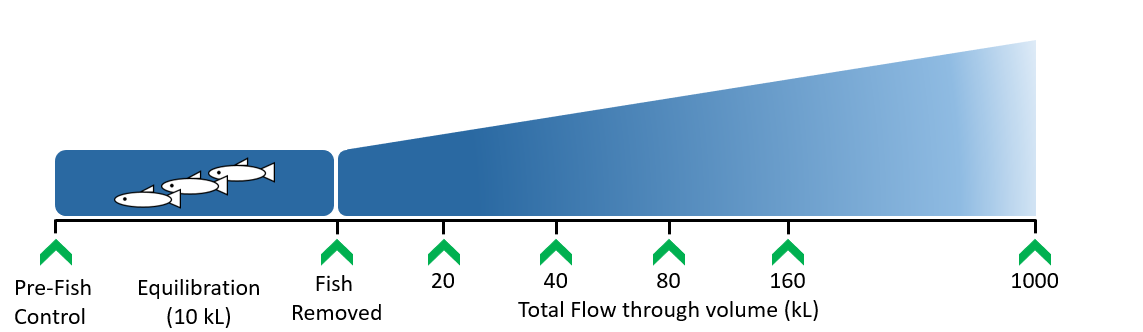
\includegraphics[scale=0.55,left]{Chapter4Images/dilutiontest.png}
\caption{ The Dilution Experiment \citep{fishforensics,hatchery}}
\label{fig:flowsamplinschedule1}
\end{figure}
		


Figure~\ref{fig:flowsamplinschedule1} depicts the dilution experiment. Three juvenile Coho salmon were placed in a minnow trap in each of four experimental tanks. The fish were left to equilibrate for nine days with flow through (140-155 L/minute). Traps containing the fish were then removed and accumulated eDNA was diluted via hatchery water flow-through. Pre-fish negative controls were collected for each tank, and fish-positive controls were collected after the nine-day equilibration period. Triplicate samples, indicated by the green arrows, at specified times representing aggregate flow-through volumes of 20, 40, 80, 160 and 1000 kL. Five negative control samples were taken concurrently from the hatchery pond (n = 3) and the hatchery kitchen sink (n= 2).

\vspace{5mm}

Each sample consisted of eight technical replicates, and each set of eight technical replicates was assigned a unique sort code. Technical replicates with sort codes equal to 31 and 84 did not pass integritE tests and were thus removed from the data set. These corresponded to samples from 20kL Flow, Tank 19 and from 1000kL Flow, Tank 20. There were an additional extra set of 12 sample replicates corresponding to 10kL Flow. These were stored in the excel file with special characters to indicate they were not to be included in analysis (because the samples had been taken after only three days, while the fish were still in the tanks opposed to after nine days). We include several tables summarizing how many samples were taken and the general method of the experiment.


\begin{table}[H]
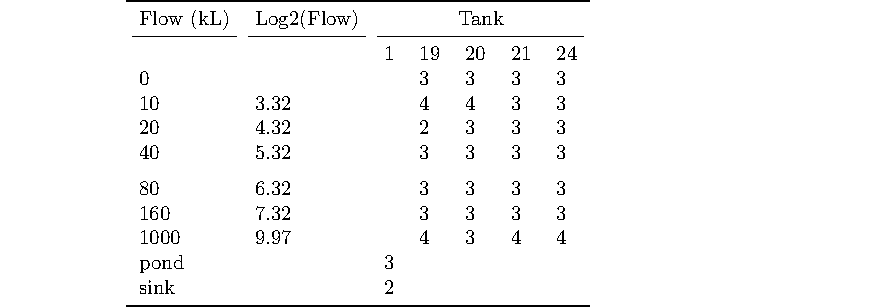
\includegraphics{Chapter4Images/flowkable1.pdf}
\caption{Summary of the number of sample replicates for each corresponding number of fish and Flow.}
\label{lab:flowkable1}
\end{table}

Table~\ref{lab:flowkable1} provides a summary of the samples taken for the dilution experiment. Also included is the number of sample replicates for sink and pond. Most levels of flow had three or four replicates taken from each tank. Two sample replicates were discarded since they did not appear to be valid measurements due to failure to pass DNA integritE tests. One was removed from tank 19 and 20kL flow and another was removed from tank 20 and 1000kL flow. The pond water had 3 sample replicates taken and the sink water had 2.
Note that for each sample replicate, there are eight associated technical replicates.



\begin{figure}[H]
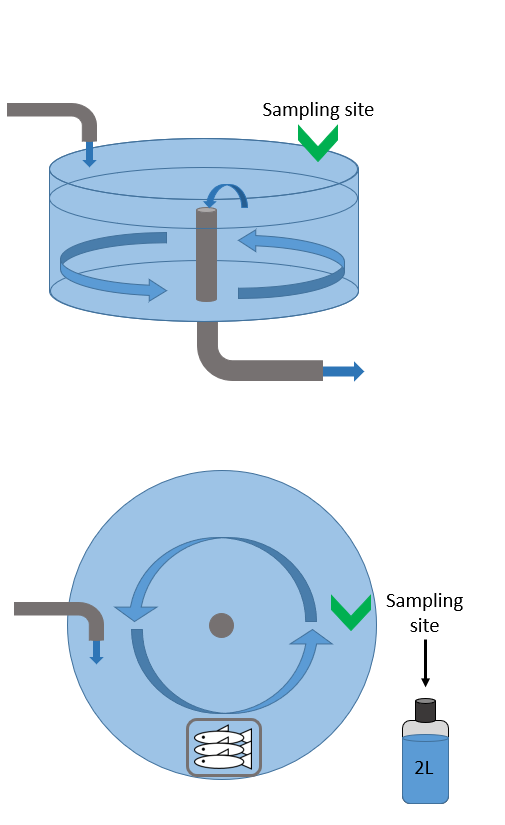
\includegraphics[scale=0.8]{Chapter4Images/flowsamplingroutinefixed.png}
\caption{Sampling routine for the flow experiment \citep{berg}.}
\label{fig:flowsamplingroutine}
\end{figure}

Figure~\ref{fig:flowsamplingroutine} represents the general method in which samples were taken. eDNA samples were taken from the opposite side of the inflow pipe. The tanks were all of size 1000kL. Three fish in a minnow trap were in each tank except for the pre-fish negative controls.



\vspace{5mm}

\begin{figure}[H]
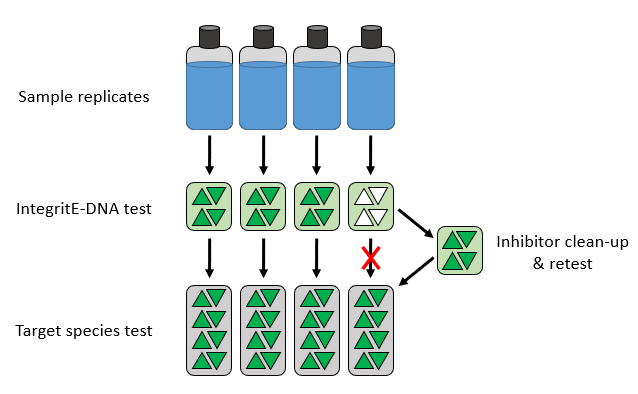
\includegraphics{Chapter4Images/flowprocedure.png}
\caption{Analysis procedure for the dilution experiment \citep{berg}.}
\label{fig:flowprocedure}
\end{figure}

Figure~\ref{fig:flowprocedure} represents the method in which quality of eDNA was assessed  before analysis. Sample replicates were first tested with integritE-DNA test. Samples which failed to pass integritE test were cleaned and retested before analysis.



